
%%% Anforderungen an die Plattform %%%
\subsection{Architecture}
\label{4b_architecture}

\begin{figure}%[btph]
    \begin{center}
        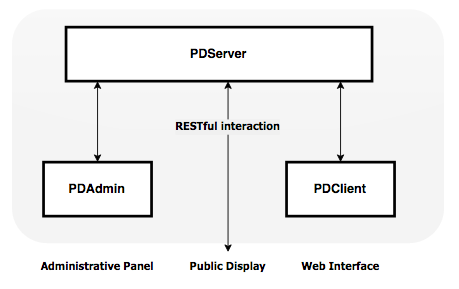
\includegraphics[width=.7\columnwidth]{img/4_implementation/4-overview}
    \end{center}
 \caption{Overview of the PDSurvey platform}
 \label{fig:4-pdsurvey-platform}
\end{figure}


The architecture for the public survey platform can be split into the following five sections:

% Overview, general requirements. Discuss all parts: 
\begin{enumerate}[itemsep=0pt] 
\item Back-end (Node.js, give reasons)
\item Front-end (Responsive)
\item API (REST)
\item Hosting
\end{enumerate}

% + state after each subsubsection why I chose which technologies and why
In the following we will first give an overview of the possible technologies and discuss why I opted for which technology.




%%  PROGRAMMING LANGUAGE  %%
\subsubsection{Programming language}

\paragraph{Categories}

\begin{enumerate}
\item Backend
\item Frontend
\item Mobile
\item Database
\end{enumerate}

% ------------------------------------- % 


\paragraph{Options}


\begin{enumerate}
\item \textbf{JavaScript}

    \begin{itemize}
        \item can be used for all platforms: front-end, back-end, public display
        \item \url{http://www.sitepoint.com/javascript-internet-things/}
        \item \textbf{Front-end}: Reasons why I chose Angular.js and not Backbone.js or Amber.js \url{https://www.airpair.com/js/javascript-framework-comparison}
        \item \textbf{Backend}: Why I chose Node.js
        \item Frameworks in Node.js: Connect, Express, Koa, ... which ones I chose why
        \item Discussion of pro/con Node.js: http://www.heise.de/developer/artikel/2x-Nein-4x-Ja-Szenarien-fuer-Node-js-2111050.html
        \item Prinzip und Verwendung von Middlewares in Node.js (wegen der Internationalisierung und Authentisierung) http://www.heise.de/developer/artikel/REST-Webservices-mit-Node-js-Teil-1-Connect-als-Fundament-1802258.html?view=print

    \end{itemize}
    
\item \textbf{Other languages}

    \begin{enumerate}
    \item PHP
    \item Python
    \item Ruby
    \item Java
    \item ASP.NET
    \end{enumerate}

\end{enumerate}
    





%%  API  %%
\subsubsection{API}

\begin{itemize}
\item REST vs SOAP
\item why I chose REST
\end{itemize}

My REST API Design, using sub-resources \url{http://code.tutsplus.com/tutorials/restful-api-design-with-nodejs-restify--cms-22637}




%%  DATABASE  %%
\subsubsection{Database}

Another fundamental aspect presented the underlying database technology, storing all of the data. A big variety of professional and open-source database management systems (DBMS) already exist on the market, but ...

Criteria for choosing the right DBMS for this project: popularity, size of community, suitability for prototyping, integration with Node.js/Angular.js

% Comparison in between ...

% My choice

Not only due to it's popularity, but also 
% - wanted to learn something new
% - popular in industry
% - MEAN stack


\paragraph{SQL: MySQL}

\begin{enumerate}
\item http://www.mysql.com/
\item "MySQL ist aus gutem Grund das Arbeitstier der Open-Source-Welt geworden: Es bietet viele der M\"oglichkeiten grosser kommerzieller Datenbanken - und ist dabei kostenlos. In seiner aktuelen Form ist MySQL performant und besitzt viele Features." \cite{hughes2012einfuhrung} (Quelle: Buch - Einf\"uhrung in Node.js, Tom Hughes-Croucher \& Mike Wilson, O'Reilly, Seite 134)
\end{enumerate}


\paragraph{SQL: PostgreSQL}

\begin{enumerate}
\item http://www.postgresql.org/
\item "Postgres (sp\"ater PostgreSQL) ist ein objektorientiertes RDBMS, das urspr\"unglich an der University of California in Berkeley entwickelt wurde. Vater des Projekts war Professor Michael Sonebraker, der es als Nachfolger seines \"alteren Ingres-Datenbank-Systems ansah. [...] Nach der Zeit in Berkeley übernahmen Open-Source-Entwickler das Projekt, ersetzten den ursprünglichen QUEL-Sprachinterpreter durch einen SQL-Sprachinterpreter und benannen das Projekt in PostgreSQL um." \cite{hughes2012einfuhrung} (Quelle: Buch - Einf\"uhrung in Node.js, Tom Hughes-Croucher \& Mike Wilson, O'Reilly, Seite 141)
\end{enumerate}


\paragraph{NoSQL: CouchDB}

\begin{enumerate}
\item http://couchdb.apache.org/
\item "CouchDB bietet einen MVCC-basierten (Multi-Version Concurrency Control) Dokumentenspeicher in einer JavaScript Umgebung. Werden Dokumente (Datens\"atze) in CouchDB hinzugef\"ugt oder aktualisiert, dann wird der gesamte Datensatz gespeichert und \"altere Versionen der Daten als obsolet markiert. Diese \"alteren Versionen des Datensazes k\"onnen immer noch in die neueste Version \"ubernommen werden, aber es wird immer eine neue Version erzeugt und f\"ur einen schnellen Lesezugriff in fortlaufenden Speicherbereichen abgelegt" \cite{hughes2012einfuhrung} (Quelle: Buch - Einf\"uhrung in Node.js, Tom Hughes-Croucher \& Mike Wilson, O'Reilly, Seite 113)
\end{enumerate}

\paragraph{NoSQL: Redis}

\begin{enumerate}
\item http://redis.io/
\item "Redis ist eine In-Memory-Datenbank mit einer Schl\"ussel/Wert-Ablage, die Ihnen sehr vertraut vorkommen sollte, wenn Sie schon \"uber Erfahrungen mit Schl\"usse/Wert-Caches wie Memcache verf\"ugen. Redis wird verwendet, wenn Performance und Skalierbarkeit wichtig sind. In vielen F\"allen entscheiden sich die Entwickler daf\"ur, es als Cache f\"ur die von einer relationealen Datenbank wie MySQL empfangenen Daten einzusetzen, auch wenn es deutlich mehr kann." \cite{hughes2012einfuhrung} (Quelle: Buch - Einf\"uhrung in Node.js, Tom Hughes-Croucher \& Mike Wilson, O'Reilly, Seite 121)
\end{enumerate}

\paragraph{NoSQL: MongoDB}

"NoSQL databases came back into the mainstream when developers needed better performance and were ok with giving up the relational aspect of RDBs (unions, joins, etc)" \url{http://psitsmike.com/2012/02/node-js-and-mongo-using-mongoose-tutorial/}

\begin{enumerate}
\item http://www.mongodb.org/
\item MongoDB is document database, storing all data in the form of JavaScript objects, PHP arrays, Python dicts or Ruby hashes. This significantly facilitates the handover from JavaScript to the database management system (DBMS).
\item "Da Mongo eine JavaScript-Umgebung mit BSON-Objektspeichern (einer Bin\"ar-Adaption von JSON) mitbringt, ist das Lesen und Schreiben von Daten aus Node heraus ausgesprochen effizient. Mongo speichert eintreffende Datens\"atze im Speicher, daher ist es in Situationen mit viel Schreibvorg\"angen eine ideale Wahl. Jede neue Version bietet verbessertes Clustering, bessere Replikation und Sharding. Da die eintreffenden Datens\"atze im Speicher abgelegt werden, ist das Einf\"ugen von Daten in Mongo nicht blockierend, womit es ideal f\"ur das Protokollieren von Operationen und Telemetriedaten ist. Mongo unterst\"utzt JavaScript-Funktionen in Abfragen. Dadurch ist es beim Lesen sehr leistungsf\"ahig, so zum Beispiel bei MapReduce-Anfragen. Mit dem dokumentenbasierten Datenspeicher von MongoDB k\"onnen Sie in Eltern-Datens\"atzen auch Kind-Datens\"atze ablegen. So kann zum Beispiel ein Blogartikel mit all seinen Kommentaren in einem einzelnen Datensatz gespeichert werden, wodurch er sich auch wieder sehr schnell auslesen l\"asst."  \cite{hughes2012einfuhrung}
\end{enumerate}

Reasons for using MongoDB
\begin{enumerate}
\item ideal for lots of write procedures
\item non-blocking write operations, ideal for Node.js and for logging data (good for our future work)
\item good read performance
\item good scalability
\item fully supports JSON syntax
\item good integration with Node.js, see Mongoose\footnote{http://mongoosejs.com/}
\end{enumerate}


Notes from the MondoDB University M101JS Class
\begin{enumerate}
\item is non-relational, ideal for JSON data
\item MongoDB is schemaless. Two documents in the same collection can have different schemas.
\item MongoDB provides a good compromise between scalability/performance and the depth of funcitonality
\item Drawback: MongoDB does not support Joins or Transactions
\end{enumerate}



%%  HOSTING  %%
\subsubsection{Hosting}

For the hosting of the platform a free and easy scalable solution was of importance. Our first choice was Heroku\footnote{https://www.heroku.com/}, due to its simplicity of setup, its native support of Node.js and the seamless integration with MongoDB\footnote{https://mongolab.com/}.

% TODO: IaaS vs PaaS: https://www.youtube.com/watch?v=Q8jZHc0NS6A
% give reasons why I chose PaaS (Platform as a Service)

    % Heroku        PaaS
    % IBM BlueMix   PaaS
    % Amawon AWS    IaaS
    % self hosting  IaaS

    %   comparison  http://smashingboxes.com/ideas/heroku-vs-amazon-web-services


Alternative were Google App Engine, IBM BlueMix, Amazon Web Services (Amazon EC2) or hosting everything on local or virtualized machines at our university. However for our scenario all of the above options had their drawbacks in comparison to Heroku. Google App Engine (as of December 2014) still had no native support for Node.js and custom runtimes had to be used to get Node.js support up and running. IBM BlueMix just got overhauled, offered full out-of-the-box Node.js support, however they only the first 30 days were free and the pricing model wasn't as attractive. Amazon Web Services offering a Infrastructure as a Service (IaaS), would have required too much administration of the server, which would have slowed down the main objective of the project, the development of the survey platform. The same goes for the last option, hosting a MEAN-stack environment on our own servers at LMU Munich. All of the above are well-known solutions in the industry, however due to simplicity and ease of use we chose Heroku.



\paragraph{Database}

http://mongoosejs.com/ + https://mongolab.com
